% THIS IS SIGPROC-SP.TEX - VERSION 3.1
% WORKS WITH V3.2SP OF ACM_PROC_ARTICLE-SP.CLS
% APRIL 2009
\documentclass{acm_proc_article-sp}

\usepackage{graphicx}
\usepackage{epsfig}
%% The amssymb package provides various useful mathematical symbols
\usepackage{amssymb}
\usepackage{amsmath}

\begin{document}

\title{Network Anomaly Detection using Co-clustering and Decision Trees}

\numberofauthors{2}

\author{
% You can go ahead and credit any number of authors here,
% e.g. one 'row of three' or two rows (consisting of one row of three
% and a second row of one, two or three).
%
% The command \alignauthor (no curly braces needed) should
% precede each author name, affiliation/snail-mail address and
% e-mail address. Additionally, tag each line of
% affiliation/address with \affaddr, and tag the
% e-mail address with \email.
%
% 1st. author
\alignauthor
Abhishek K Srivastava \\
       \affaddr{University of California,Riverside}\\
       \affaddr{900 University Ave,}\\
       \affaddr{Riverside, CA, 92521}\\
       \email{asriv003@ucr.edu}\\
}
\maketitle
\begin{abstract}
In current times it is very important to maintain a high level security to ensure safe and trusted communication of information for multiple purposes. But secured data communication over internet and any other network is always under threat of intrusions and misuses. There is certainly various interest lies on how to classify between bad connection from normal ones. So Network anomaly detection have become a needful component in terms of computer and network security.

In my project i used a well known technique known as ``co-clustering'' with decision trees for the evaluation of the classification of the connections. My evaluation shows that we can certainly use clustering techniques with other methods for detecting and finding very interesting patterns in network connections.

\end{abstract}

\section{Introduction}
As network systems get more complex by the day and new technologies emerge at a rapid pace, the vulnerabilities they are prone to also increases. The current systems/software in place for detecting network intrusions or anomaly connections would not be able to prevent all types of attacks as new types appear. The act of detecting actions that attempt to compromise the integrity, confidentiality, or availability of a computer resource can be referred as intrusion detection. Present firewalls and other such mechanism rely on certain properties of a connection to determine if that connection is a normal or a malicious connection\cite{lrr}. 

Thats why there is a need of adaptive network anomaly detection using machine learning which can easily adapt to the newer attacks by learning their properties. An network anomaly detection system is a device or software application that monitors network and/or system activities for malicious activities or policy violations and produces reports\cite{kdm}

From the perspective of the end users the security issue creates the challenge for system administrators on how to distinguish normal connections of legitimate users from malicious connections. An administrator, in the face of an attack, wants to block such malicious connections without blocking legitimate users. We can never know for sure if any given connection is legitimate or malicious, but we can attempt to isolate a set of connections that stand out from normal user behavior, so as to help system administrators detect attacks. Anomaly detection specifically handles these situations.

In my project i used data set provided by KDD in 1999 for designing systems for intrusion detector learning task whose objective was to build a predictive model (i.e. a classifier) capable of distinguishing between ``bad'' connections, called intrusions or attacks, and ``good'' normal connections.\cite{kdd}

In this project i analyze a given set of connection measurements, each of which consists of a set of connection parameters categorize each connection as ``normal'' or ``anomalous''. Based on this data design a classifier which can learn and predict the connection type solely on these set of parameters. I built the classifier predominantly using following techniques:
\begin{itemize}
\item Co-Clustering
\item Decision Trees
\end{itemize}

After training the classifier i tested it with the test set and although there was not much increase in the accuracy of the data but it did pacified few of the shortcomings of the previous systems.

The outline of the paper is as follows. In Section 2 I describe our related work done with some motivation for pursuing co-clustering and decision trees as my method of analyzing this data. In Section 3 we describe the implementation for the data mining techniques i used, explaining the reason for choosing certain parameters and methods. In Section 4 i give the results of running numerous experiments using the implemented methods and algorithms. Finally, in Section 5 i describe the conclusions of the project and about the usefulness of method i used and how the two algorithms used together to detect and analyze anomalous connections can be useful followed by the future work and what extension can be made to this model.

\section{Related Work}
Since instrusion detection is very popular field of interest among researchers various work have already been done on these topics. I won't be mentioning all of them but only those who provided motivation for doing this project.

The major motivation for the project was provided by paper \textbf{Network Anomaly Detection using Co-clustering} and my project was an extension of this paper by taking it as a base and extending with a different models. In this paper authors presents two ways of doing co-clustering: SMR co-clustering \& Information theoretic co-clustering(can be read in detail from the paper) and put argument that using these techniques helps in identifying task with good certaintity. Co-clustering may be described as follows: Given a data matrix, we seek to find subsets of rows that are correlated with only a subset of its columns as opposed to the traditional clustering approach, where a subset of the rows has to be similar across all columns/dimensions. Since there is an intuition to apply ``co-clustering'' for detecting network anomalies because there are certain set of anomalies depend on different set of parameters, co-clustering them and extracting information from those clusters can be used to extend it to other models. That was the prime motivation for me to use ``Co-clustering'' as a basis for this project. And this method easily applies to the problem at hand, where we model the set of connection measurements as a matrix, where the rows correspond to each distinct connection, and the columns corresponds to the connection's parameters. \cite{papal} 

The paper also claims that ``PCA'' a well known technique for standard dimensionality reduction, which enables us to visualize high dimensional data \cite{pca}. But it does not provide very good results as seen in the Figure 1. It plot was plotted by applying to the data and first two components were selected and plotted. We observe that normal and anomalous connections cannot be clearly differentiated without the labels. 

\begin{figure}
\centering
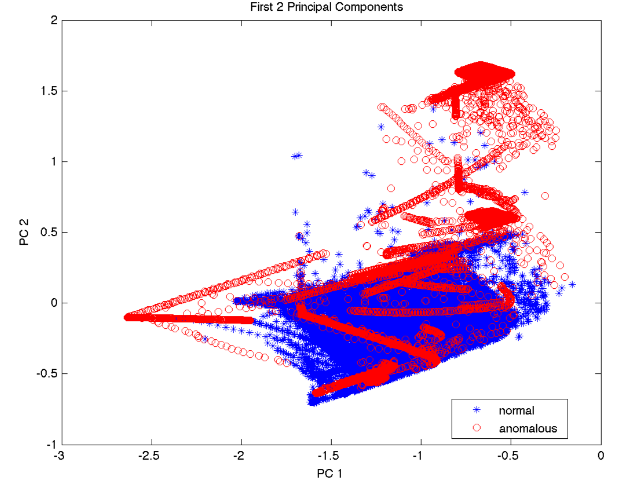
\epsfig{file=np_10.png, height=2.5in, width=2.85in}
\caption{Plot of first two PCA.}
\end{figure}

The motivation for using decision tree was because of the simplicity of the classifier and one of the entries for this KDD competition which won it used the method called ``Bagged Boosting'' as a classifier, which was a modified version of decision trees\cite{bbt}. This shows that standalone decision trees with modification can also perform better for this classification task and this dataset. My project did not use any version of the model presented in the paper but rather simpler version of decision tree.
\begin{figure}[h]
	\centering
	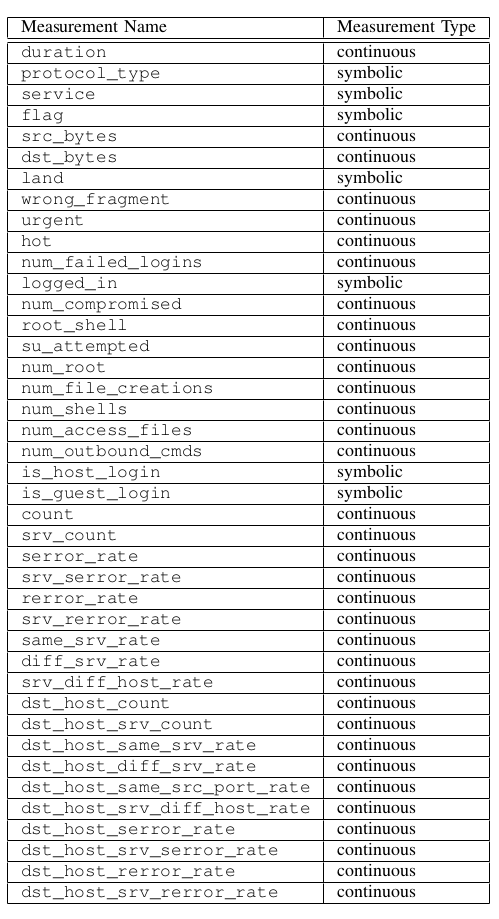
\epsfig{file=np_1_1_1.png, height=4.9in, width=2.25in}
	\caption{List of connections measurements in the data set.}
\end{figure}
\section{Implementation}
Steps involved during the implementation of this project will be explained in the following subsections.

\subsection{Data Preprocessing}

The data obtained for this project was already very clean and had no missing data so not much effort needed for that. I used the labeled portion of the dataset, which consists of 494020 connections; 97277 out of them are ``normal'' and 396743 are ''attacks''. For each connection there are 37 recorded measurements, listed in Figure 2. There are 22 different types of attacks in the labeled data set but those were mapped to only 5 labels. Mapping all 22 attacks to the 5 labels in shown in the Figure 3.

The data consists of both discrete and continuous values, discrete values being string values. So the main issue i faced while working with the project is converting the data from discrete string values to the categorical integer values. For some features number of discrete string can be upto 65. Converting test data to trained format was even more challenging because in the test data there are additional 16 attacks which needed to be classified into 5 main category. Other than these issues there are no additional pre-processing required for this data set.

\begin{figure}
\centering
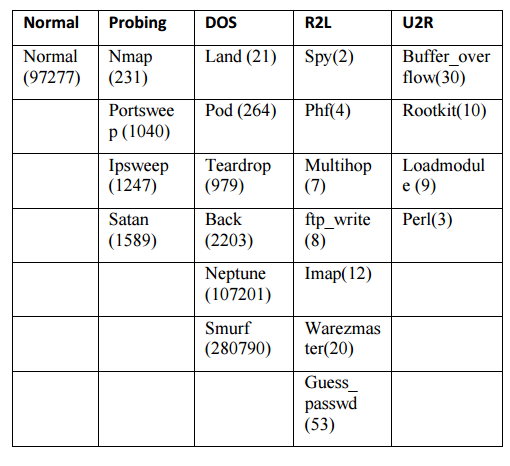
\epsfig{file=np_2_1.png, height=2.75in, width=3in}
\caption{Mapping of different labels into different attack types.}
\end{figure}

\begin{figure}
	\centering
	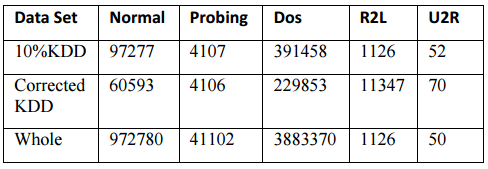
\epsfig{file=np_3_1.png, height=1.0in, width=3in}
	\caption{Dstribution of intrusion types in datasets.}
\end{figure}
\subsection{Classifier Implementation}
For the implementation part i choose to use Information theoretic co-clustering \cite{itcc} which a hard co-clustering method. Reason for choosing hard co-clustering is identifying specifically which parameters are clustered together in disjoint way and there is no overlapping between. The code was available for this co-clustering methods by the author of this paper and also few packages were available. But i implemented the code in python taking the reference of julia code. The  function calling convention was:


$M$, $q$, $cX$, $cY$, $err$  = ITCC($d$, $k$, $l$, $n\_i$, $c\_th$, $cX$, $cY$)


$d$: Data need to be clustered, $k$: Number of row-clusters, $l$: Number of column-clusters, $n\_iters$: Maximum number of iterations, $c\_th$:Converge threshold at which algorithm has is said to have converged, i.e. KL-D between p and q has not decreased significantly between iterations, $cX$: Initial row-cluster assignments (default to random assignments), $cY$: Initial column-cluster assignments (also default to random assignments). The results we get are $M$: View of data given final cX and cY, $q$: Final conditional probability distribution, $cX$: Final row-cluster assignments, $cY$: Final column-cluster assignmnents, $err$ : Final Kullback-Leibler divergence error between p and q.

\subsection{Result Processing}
After getting the results $cX$ \& $cY$ i use them to reduce the features from the original data and then use the reduced feature to build the decision tree classifier. For testing the results of test data modify it as well based on $cX$ and $cY$ and do the prediction by running it through the trained model and calculate the confusion matrix which is the testing parameter for this project and reason for doing this is explained in the following section.

\section{Result and Findings}
The reason for choosing confusion matrix was because calculating the accuracy was not correct predictive model for it. Data was skewed for some of the classes so accuracy does not represent correct predictive nature of the model. Each column of the matrix represents the instances in a predicted class while each row represents the instances in an actual class (or vice versa). I did a comparison with the confusion matrix of 1-NN classifier due the fact that it is the most basic method of solving this problem and to be considered as base to improve upon. Table of confusion matrix for both 1-NN model and Co-clustering with decision tree model is given in table 1 and table 2. 

\begin{table}
	\centering
	\caption{Confusion Matrix of 1-NN.}
	\begin{tabular}{|c|c|c|c|c|c|l|} \hline
		Actual/Pred.&Norm&Prob&Dos&r2l&u2r&\%Corr\\ \hline
		Normal&60322&212&57&1&1&99.6\% \\ \hline
		Probing&697&3125&342&0&2&75.0\% \\ \hline
		Dos&6144&76&223633&0&0&97.3\% \\ \hline
		r2l&209&5&1&8&5&3.5\% \\ \hline
		u2r&15785&308&1&0&95&0.6\% \\ \hline
	\end{tabular}
\end{table}

\begin{table}
	\centering
	\caption{Confusion Matrix of Co-clustering with AdaBoost.}
	\begin{tabular}{|c|c|c|c|c|c|l|} \hline
		Actual/Pred.&Norm&Prob&Dos&r2l&u2r&\%Corr\\ \hline
		Normal&42138&1421&15835&486&713&69.5\% \\ \hline
		Probing&921&432&228489&2&149&71.1\% \\ \hline
		Dos&6144&76&223633&0&0&97.3\% \\ \hline
		r2l&209&5&1&8&5&3.5\% \\ \hline
		u2r&15785&308&1&0&95&0.6\% \\ \hline
	\end{tabular}
\end{table}

I am listing few of the findings below i observed from the data set with my model and compared against 1-NN model.
\begin{itemize}
	\item The accuracy for predicting normal connection reduced from the basic model for which there can be multiple reasons. The first one can be observed that prediction for ``Dos'' attack went up which means that the model did get over-fitted for that test case and due to that accuracy of the model went down for normal connections which can be observe since the prediction for ``Dos'' attack went up for each class. Same thing can be observed for probing attack which also got downgraded. The other reason can be co-clustering did not performed good for the normal connections with only ~75\% purity which can get extended to the decision tree model.
	\item On the bright side my model did performed well for the skewed classes. R2L and U2R attack accuracy was very bad in the 1-NN model but using my model it shows a get improvement for those attacks. Which is clearly evident that co-clustering did able to cluster features for those attack better than the base model.
	\item Another reason for bad performance of this model was distribution of classes for both train data and test data to be different. Few experiments would have given me better answers but not able to perform them. Few cases i have in my mind is do a sampling from the actual data to train them with multiple batches over multiple iterations which can help find better features to work with and that can lead to better performance of the classifier as well. But this will be very expensive since co-clustering time cost is very high and running multiple iteration can take quite a while to train them. Another experiment i wanted to try was training the model where data have approximately same distribution but this wont be a good idea since sample size of other attacks are not very large and training data will be very small to train the model in a good way.
\end{itemize}

\section{Future Work}
There is a lot of work/experiments can be done to improve this project or gain more insights on how to improve the model. Few of them i think of which can might work are listed below:
\begin{itemize}
	\item Using a soft co-clustering method: This is a total experimental claim. Although the original paper do claim to perform better than the hard co-clustering how it will perform with the decision tree model is i cannot say or claim. 
	\item Fine tuning: This is also a optional things to do. Many of the parameter which were used in the ITCC method were set instinctively and which can be tuned to give better model. Some of the parameters which are being passed as a random value although have less implication but can give a bad clustering. There is also uncertainty with  data since it always used some approximation to generate conditional probability distribution which is used further for co-clustering and can result in a bad local minima. 
	\item GLM co-clustering: It is also a not certain claim but using a different co-clustering method can perform better that ITCC method. In the GLM co-clustering paper is is claimed by the author that this co-clustering method is less susceptible to the distribution of the classes in the training and testing data which can certainly help given our dataset property\cite{glm}. 
\end{itemize}

\section{Conclusions}
After completing all the steps mentioned above we can conclude that although the model i used in not perfect but it did improve on some things. It was able to better classify the classes with skewed data it means that it is able to capture few of the properties correctly for those classes. Aslo co-clustering by itself is a wonderful technique to be used for clustering data in better way for these kind of data where PCA does not work that well. 

The other improvement i will discuss is better performance of the model with respect to the time. Testing data for co-clustering is equally time consuming task as the training the data. Which my proposed model do able to pacify but with some accuracy trade-off.

\begin{thebibliography}{9} 
	\bibitem{lrr}Lalindra De Silva, Ravindra Aditya Varma, Raghav Aggarwal. \emph{``Improving Network Intrusion Detection Through Classifier Combination''.} School of Computing, University of Utah, Salt Lake City.\\
	
	\bibitem{kdm}K. Scarfone, P. Mell. \emph{``Guide to Intrusion Detection and Prevention Systems (IDPS)''.}  Security Resource Center (National Institute of Standards and Technology).\\
	
	\bibitem{kdd}KDD Cup 1999 Data: \emph{Data set used for The Third International Knowledge Discovery and Data Mining Tools Competition.}\\
	
	\bibitem{papal} Evangelos E. Papalexakis, Alex Beutel, Peter Steenkiste. ASONAM '12 \emph{``Network Anomaly Detection using Co-clustering''.}\\
	
	\bibitem{pca} Svante Wold, Kim Esbensen and Paul Geladi. 1987 \emph{``Principal Component Analysis''.} Chemometrics and Intelligent Laboratory \\
	
	\bibitem{bbt} Bernhard Pfahringer SIGKDD'2000. \emph{``Winning the KDD99 Classification Cup: Bagged Boosting''.} Austrian Research Institute for AI, Vienna, Austria.\\
	
	\bibitem{itcc}Inderjit S. Dhillon, Subramanyam Mallela, Dharmendra S. Modha KDD'03. \emph{``Information-Theoretic Co-clustering''.} Dept. of Computer Sciences
	University of Texas, Austin.\\
	
	\bibitem{glm}Zhanpan Zhang, Daniel R. Jeske, Xinping Cui, Mark Hoddle JABES'12. \emph{``Co-clustering Spatial Data Using a Generalized Linear Mixed Model With Application to the Integrated Pest Management''.} Department of Statistics, University of California Riverside.\\
\end{thebibliography}

% That's all folks!
\end{document}